\scanpage{19}
des fibres $I_\alpha$ et $\widetilde A_\alpha$ de $I$ et $A$ au dessus de $\alpha$. La donnée d'une courbe \unsure{standard|standart} $G$ épinglée sur $\mathcal S$ équivaut à la donnée, \deleted{de} pour $\forall\ \alpha\in S$, d'une courbe relative (propre lisse \inserted{relt} $0$-connexe) $Y_\alpha$ sur $\mathcal S$, de genre relatif $g_\alpha$, \uline{et} d'un \inserted{$\mathcal S$-}mono. $(\widehat I_\alpha)_{\mathcal S}\hookrightarrow Y_\alpha$.

Désignons, \deleted{par $\mathcal M_{g_\alpha,\deleted{\nu_\alpha}\inserted{\widehat I_{\unsure{\alpha}}}}$} pour \deleted{\unsure{de}}\inserted{un} entier naturel $g\deleted{\unsure{\alpha}}$ et un ens. fini $I$ (de cardinal $\nu$) par
\figure{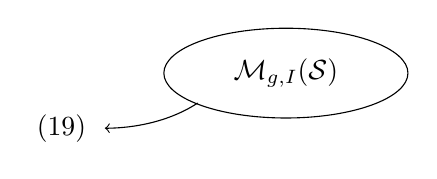
\begin{tikzpicture}[baseline=(m.base)]
\node (m) at (0,0) {$\mathcal M_{g,I}(\mathcal S)$};
\draw (0,0) ellipse (1.55 and .57);
\draw[->] (-1.12,-.38) .. controls (-1.55,-.66) and (-2.05,-.7) .. (-2.3,-.7);
\node at (-2.85,-.7) {$(19)$};
\end{tikzpicture}}
le \deleted{catégorie}\inserted{groupoïde} des courbes relatives $Y$ (propres, lisses, $0$-connexes) sur $\mathcal S$, \uline{$I$-ponctuées} i.e. munies d'un mono. $I_{\mathcal S}\hookrightarrow Y$. On trouve donc, si
\[
(20)\qquad\mathcal M_G(\mathcal S)
\]
désigne le groupoïde des courbes \unsure{standard|standart} $G$-épinglées sur $\mathcal S$, une équivalence
\[
(21)\qquad\mathcal M_G(\mathcal S)\simeq\prod_{\alpha\in S}\mathcal M_{g_\alpha,\widehat I_\alpha}(\mathcal S).
\]
\mspage{18}
